\documentclass[12pt]{article}
\usepackage{amsmath}
\usepackage{amsfonts}
\usepackage{amssymb}
\usepackage{geometry}
\usepackage{graphicx}
\geometry{a4paper, margin=0.8in}
\pagenumbering{gobble}

\title{Homework assignment for 02YMECH \\ Chapter: Oscillations}
\begin{document}
\date{}
\maketitle
\vspace{-0.8in}

\begin{enumerate}
    \item The position of a particle hooked to a spring is given by the equation \( x(t)=A \cos(\omega_0 t + \phi) \), where \( A \), \( \omega_0 \), and \( \phi \) are constants. If the particle's initial position is $x_0$ and initial velocity is $v_0$, how long will it take for the particle to reach its maximum displacement for the first time?
    \item What is the average kinetic energy and average potential energy of a harmonic oscillator over one complete cycle? Express your answers in terms of the total energy \( E \) of the system.(Consider the time integrals of kinetic and potential energy over one period.)
    \item A simple pendulum consists of a bob of mass $m$ attached to a light, inextensible string of length $L$, staying in its equilibrium position. The support point of the pendulum is suddenly accelerated horizontally with constant acceleration $a$ (e.g., the ceiling begins to move to the right). 
    \begin{enumerate}
        \item Determine the new equilibrium angle \( \theta \) that the pendulum makes with the vertical.
        \item Find the period of small oscillations about this new equilibrium position.
    \end{enumerate}
    \item The position of a damped harmonic oscillator is given by the equation \( x(t) = A e^{-\beta t} \cos(\omega_1 t + \phi) \), where \( A \), \( \beta \), \( \omega_1 \), and \( \phi \) are constants. How much time will it take for the amplitude of the oscillations to decrease to half of its initial value?
    \item Calculate the average total mechanical energy of driven damped harmonic oscillator over one complete cycle. Calculate the total energy when the driving frequency is equal to the natural oscillation frequency.
    \item Calculate the power delivered by the driving force to the damped harmonic oscillator. Show that, on average, it is equal to the power dissipated by the frictional force.
    \item Express the total energy of the damped harmonic oscillator in terms of time \( t \), quality factor \( Q \) and natural oscillation frequency \( \omega_0 \). Interpret the result.
    \newpage
    \item Consider the following two diagrams:
\vspace{0.4cm}

\begin{minipage}{0.49\textwidth}
\centering
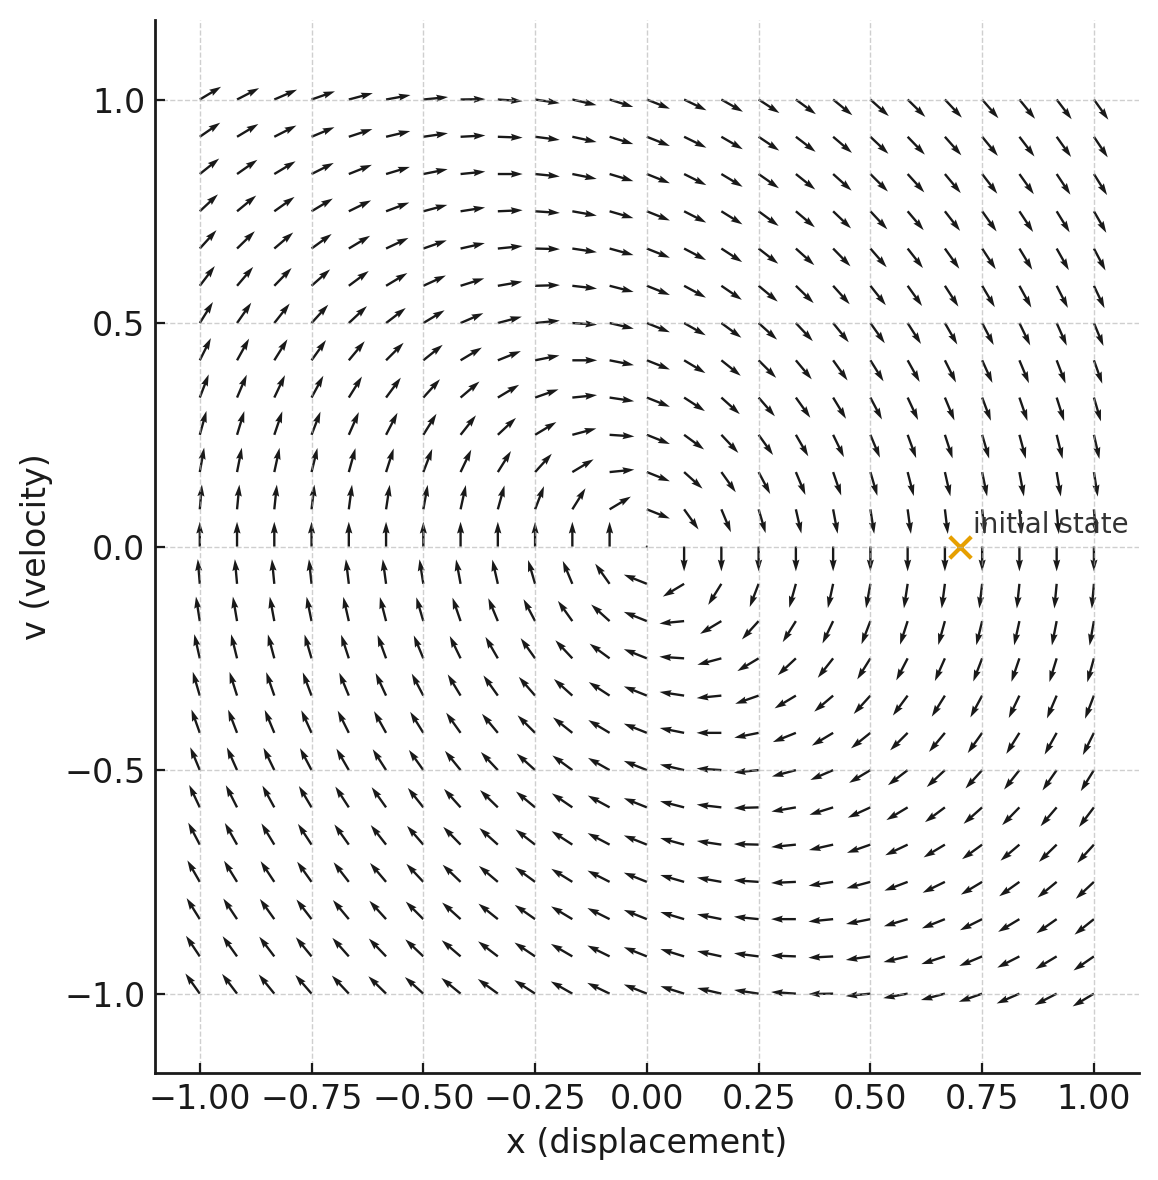
\includegraphics[width=\linewidth]{do.png}
\end{minipage}\hfill
\begin{minipage}{0.49\textwidth}
\centering
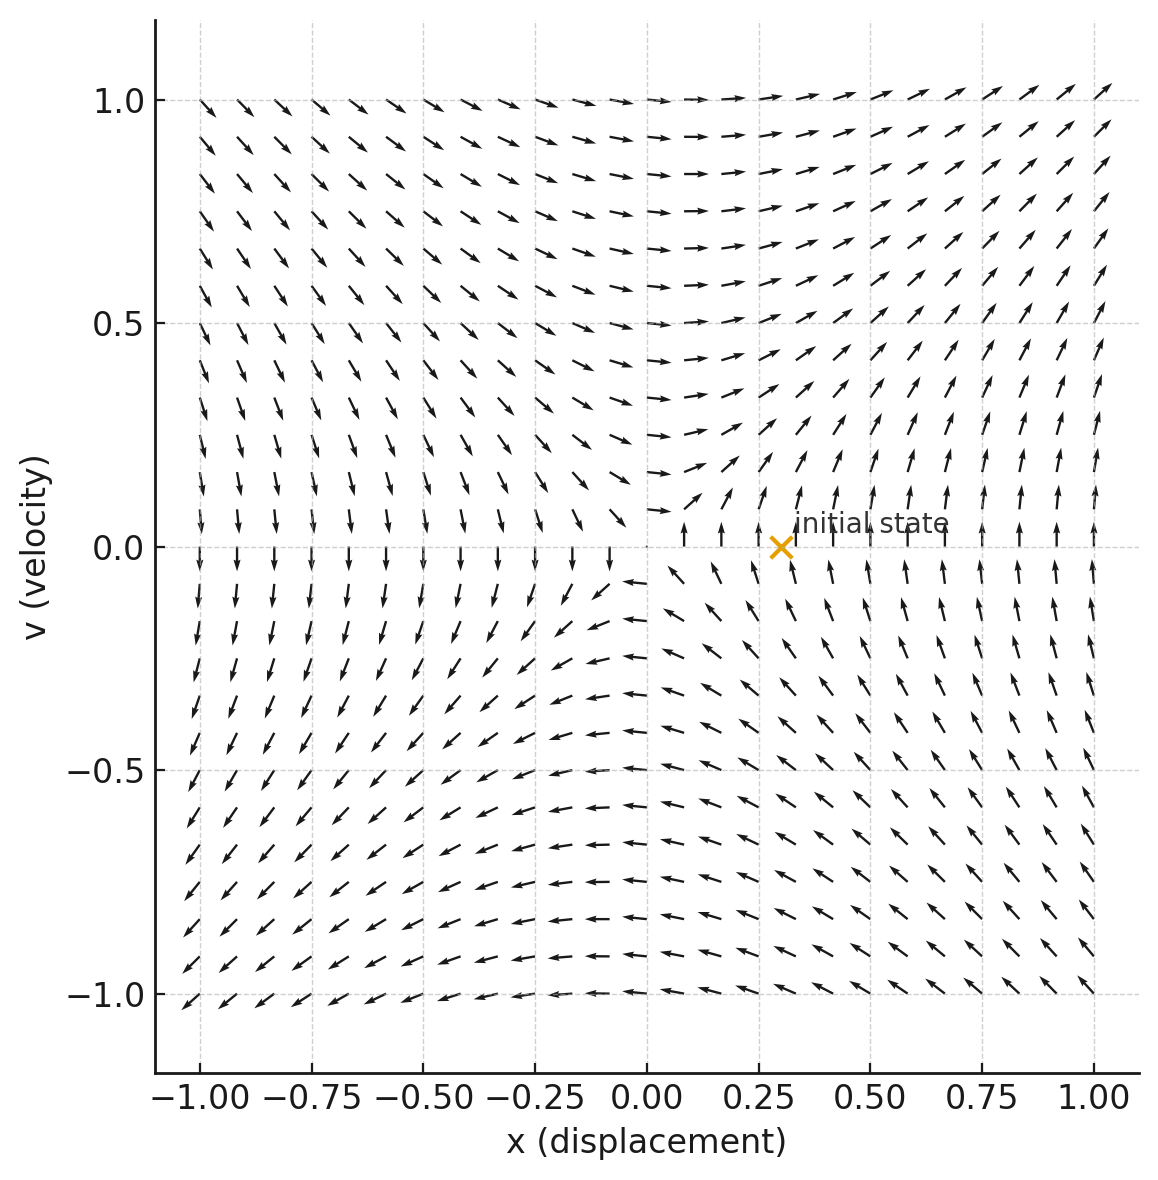
\includegraphics[width=\linewidth]{ip.png}
\end{minipage}

\vspace{0.5cm}
\noindent
Comment on the time evolution of the system in both the cases concisely. Which one would you classify as stable and which one as unstable? Justify your answer.

\end{enumerate}
\end{document}
